\subsubsection{ Counter write }

\begin{itemize}

    \item For each $i = 1,2,3$,
                   $j = l-1,\ldots,1$,
                   $u \in \{0, 1\}^j$, and each
                   $\inc \in \{{\tt increment}, {\tt copy} \}$:
        \begin{itemize}
        \item Create
        $\begin{aligned}[t]
            \cwrite(& \left\langle {\tt CounterWrite}, i, u0, \inc \right\rangle,
                      \left\langle {\tt CounterWrite}, i, u,  \inc \right\rangle \;)
        \end{aligned}$ \\ from the general gadget in Figure~\ref{fig:counter_write_0}

        \item Create
        $\begin{aligned}[t]
            \cwrite(& \left\langle {\tt CounterWrite}, i,  u1, \inc \right\rangle,
                      \left\langle {\tt CounterWrite}, i,  u,  \inc \right\rangle \;)
        \end{aligned}$ \\ from the general gadget in Figure~\ref{fig:counter_write_1}


        \item Create
        $\begin{aligned}[t]
            \cwrite(& \left\langle {\tt CounterWrite}, 1, u0, \inc, {\tt msr} \right\rangle,
                      \left\langle {\tt CounterWrite}, 1, u,  \inc, {\tt msr} \right\rangle \;)
        \end{aligned}$ \\ from the general gadget in Figure~\ref{fig:counter_write_0}

        \item Create
        $\begin{aligned}[t]
            \cwrite(& \left\langle {\tt CounterWrite}, 1,  u1, \inc, {\tt msr} \right\rangle,
                      \left\langle {\tt CounterWrite}, 1,  u,  \inc, {\tt msr} \right\rangle \;)
        \end{aligned}$ \\ from the general gadget in Figure~\ref{fig:counter_write_1}

        \item Create
        $\begin{aligned}[t]
            \cwrite(& \left\langle {\tt CounterWrite}, i, u0, \inc, {\tt msr}, {\tt msd} \right\rangle,
                      \left\langle {\tt CounterWrite}, i, u,  \inc, {\tt msr}, {\tt msd} \right\rangle \;)
        \end{aligned}$ \\ from the general gadget in Figure~\ref{fig:counter_write_0}

        \item Create
        $\begin{aligned}[t]
            \cwrite(& \left\langle {\tt CounterWrite}, i,  u1, \inc, {\tt msr}, {\tt msd}\right\rangle,
                      \left\langle {\tt CounterWrite}, i,  u,  \inc, {\tt msr}, {\tt msd}\right\rangle \;)
        \end{aligned}$ \\ from the general gadget in Figure~\ref{fig:counter_write_1}
        \end{itemize}

    \item For each $i = 1,2,3$ and each $\inc \in \{{\tt increment}, {\tt copy} \}$:
    \begin{itemize}
        \item Create
        $\begin{aligned}[t]
            \cwrite(& \left\langle {\tt CounterWrite}, i, 0, \inc \right\rangle,
                      \left\langle {\tt DigitTop},     i,    \inc \right\rangle \;)
        \end{aligned}$ \\ from the general gadget in Figure~\ref{fig:counter_write_0}

        \item Create
        $\begin{aligned}[t]
            \cwrite(& \left\langle {\tt CounterWrite}, i, 1, \inc \right\rangle,
                      \left\langle {\tt DigitTop},     i,    \inc \right\rangle \;)
        \end{aligned}$ \\ from the general gadget in Figure~\ref{fig:counter_write_1}

        \item Create
        $\begin{aligned}[t]
            \cwrite(& \left\langle {\tt CounterWrite}, 1, 0, \inc, {\tt msr} \right\rangle,
                      \left\langle {\tt DigitTop},     1,    \inc, {\tt msr} \right\rangle \;)
        \end{aligned}$ \\ from the general gadget in Figure~\ref{fig:counter_write_0}

        \item Create
        $\begin{aligned}[t]
            \cwrite(& \left\langle {\tt CounterWrite}, 1, 1, \inc, {\tt msr} \right\rangle,
                      \left\langle {\tt DigitTop},     1,    \inc, {\tt msr} \right\rangle \;)
        \end{aligned}$ \\ from the general gadget in Figure~\ref{fig:counter_write_1}

        \item Create
        $\begin{aligned}[t]
            \cwrite(& \left\langle {\tt CounterWrite}, i, 0, \inc, {\tt msr}, {\tt msd}\right\rangle,
                      \left\langle {\tt DigitTop},     i,    \inc, {\tt msr}, {\tt msd}\right\rangle \;)
        \end{aligned}$ \\ from the general gadget in Figure~\ref{fig:counter_write_0}

        \item Create
        $\begin{aligned}[t]
            \cwrite(& \left\langle {\tt CounterWrite}, i, 1, \inc, {\tt msr}, {\tt msd}\right\rangle,
                      \left\langle {\tt DigitTop},     i,    \inc, {\tt msr}, {\tt msd}\right\rangle \;)
        \end{aligned}$ \\ from the general gadget in Figure~\ref{fig:counter_write_1}
    \end{itemize}

\end{itemize}

\vspace{.5cm}

\begin{figure}[H]
    \centering
    \subcaptionbox{{\tt Counter\_Write\_0} \label{fig:counter_write_0}}
    {\makebox[0.24\textwidth][c]{
\includegraphics[width=0.45in]{counter_write_0}}}%
    ~
    \subcaptionbox{{\tt Counter\_Write\_1} \label{fig:counter_write_1}}
    {\makebox[0.24\textwidth][c]{
\includegraphics[width=0.45in]{counter_write_1}}}%
    ~
    \subcaptionbox{Digits 1, 2, \& 3 -\\ general overview\label{fig:counter_write_i_op}}
    {\makebox[0.24\textwidth][c]{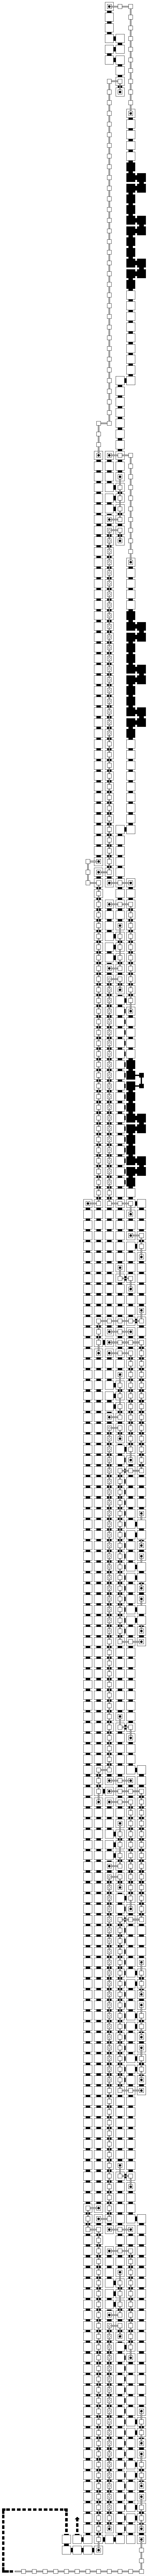
\includegraphics[width=0.45in]{overviews/general/counter_write_i_op}}}%
    ~
    \subcaptionbox{Digits 1, 2, \& 3 -\\ general (seed) overview\label{fig:counter_write_i_seed_op}}
    {\makebox[0.24\textwidth][c]{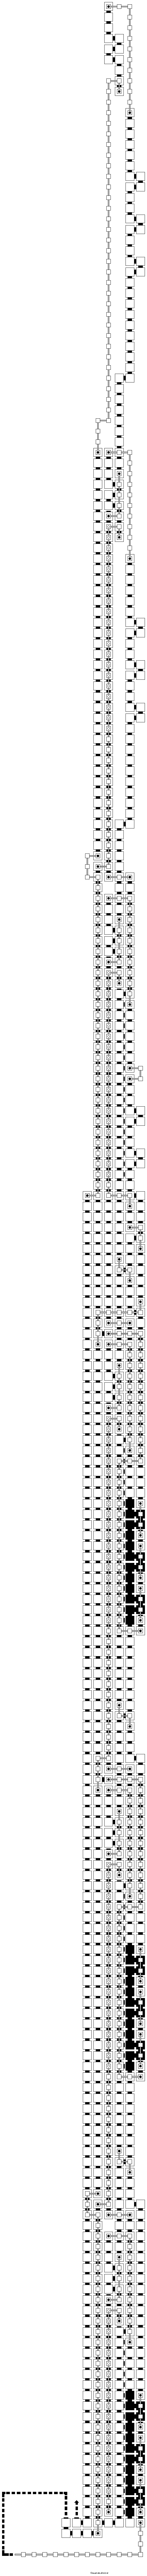
\includegraphics[width=0.45in]{overviews/general/counter_write_i_seed_op}}}%
    ~
\end{figure}

\begin{figure}[H]\ContinuedFloat
    \centering
    \subcaptionbox{Digit 1 -- case 1\label{fig:counter_write_1_op_msr_msd}}
    {\makebox[0.24\textwidth][c]{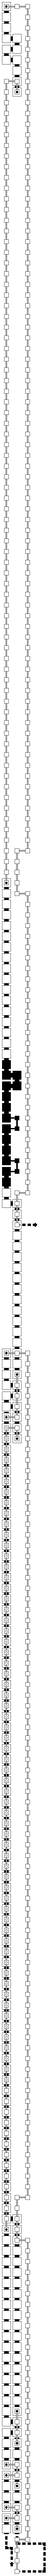
\includegraphics[width=0.45in]{overviews/case1/counter_write_1_op_msr_msd}}}%
    ~
    \subcaptionbox{Digit 1 -- case 1 (seed)\label{fig:counter_write_1_op_seed_msr_msd}}
    {\makebox[0.24\textwidth][c]{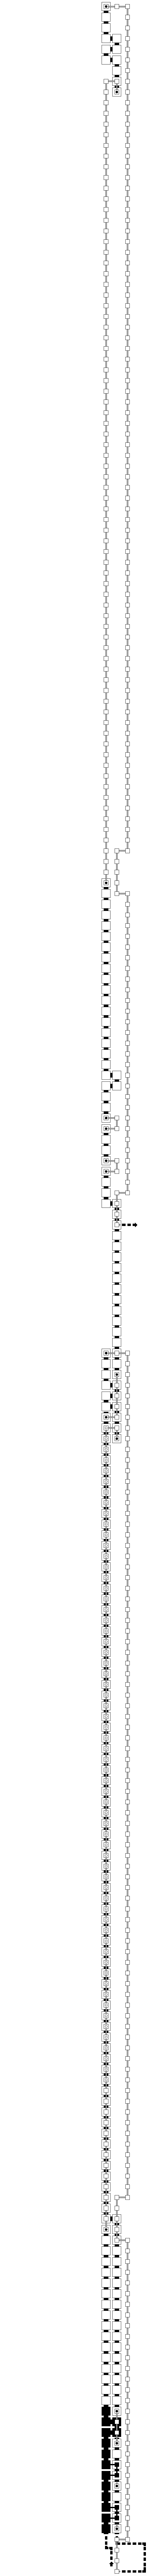
\includegraphics[width=0.45in]{overviews/case1/counter_write_1_seed_op_msr_msd}}}%
    ~
    \subcaptionbox{Digit 1 -- case 2\label{fig:counter_write_1_op_msr}}
    {\makebox[0.24\textwidth][c]{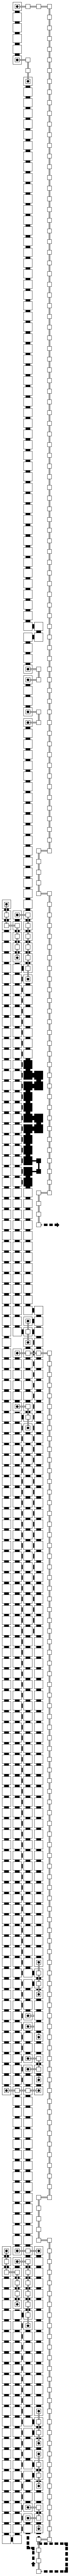
\includegraphics[width=0.45in]{overviews/case2/counter_write_1_op_msr}}}%
    ~
    \subcaptionbox{Digit 1 -- case 2 (seed)\label{fig:counter_write_1_op_seed_msr}}
    {\makebox[0.24\textwidth][c]{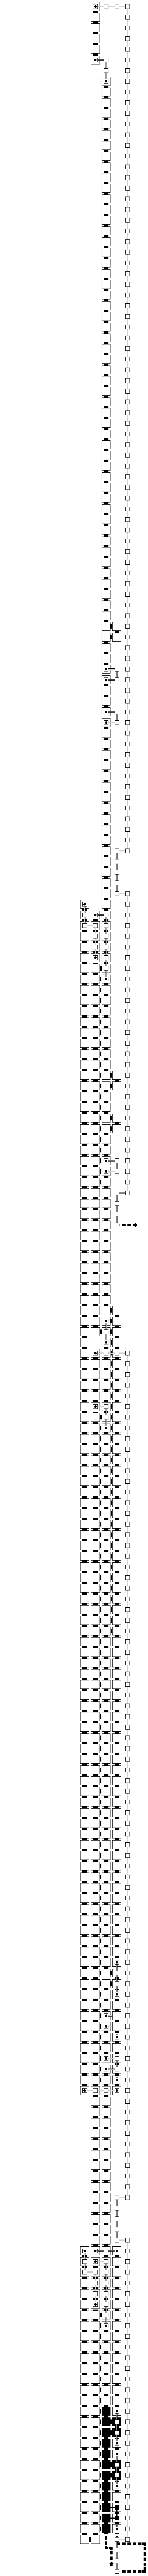
\includegraphics[width=0.45in]{overviews/case2/counter_write_1_seed_op_msr}}}%
    ~
\end{figure}

\begin{figure}[H]\ContinuedFloat
    \centering
    \subcaptionbox{Digit 2 -- case 2 \label{fig:counter_write_2_op_msr_msd}}
    {\makebox[0.24\textwidth][c]{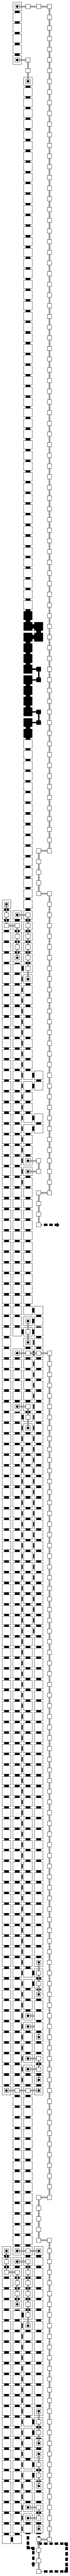
\includegraphics[width=0.45in]{overviews/case2/counter_write_2_op_msr_msd}}}%
    ~
    \subcaptionbox{Digit 2 -- case 2 (seed)\label{fig:counter_write_2_op_seed_msr_msd}}
    {\makebox[0.24\textwidth][c]{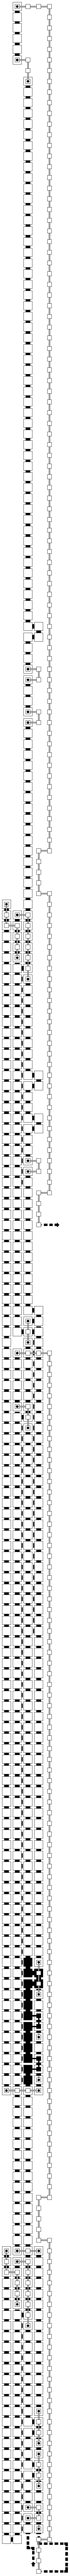
\includegraphics[width=0.45in]{overviews/case2/counter_write_2_seed_op_msr_msd}}}%
    ~
    \caption{\label{fig:counter_write} The {\tt Counter\_Write} gadgets}
\end{figure}